\section{Introduction to Neural Networks}

Neural Networks are a type of a machine learning model inspired by activities in human brain.
A neural network comprises of `neurons`, which are considered as the building blocks.
A neuron in a neural network is implemented as weighted sum of its input, which is then passed through a non-linear function. This non-linear function is often denoted as an activation function and most commonly is a sigmoid or a rectified linear function.

Let $W$ be weights and $x$ denote the inputs. Let $g$ be the activation function, then a single neuron is represented as - 


\begin{figure}[H]
   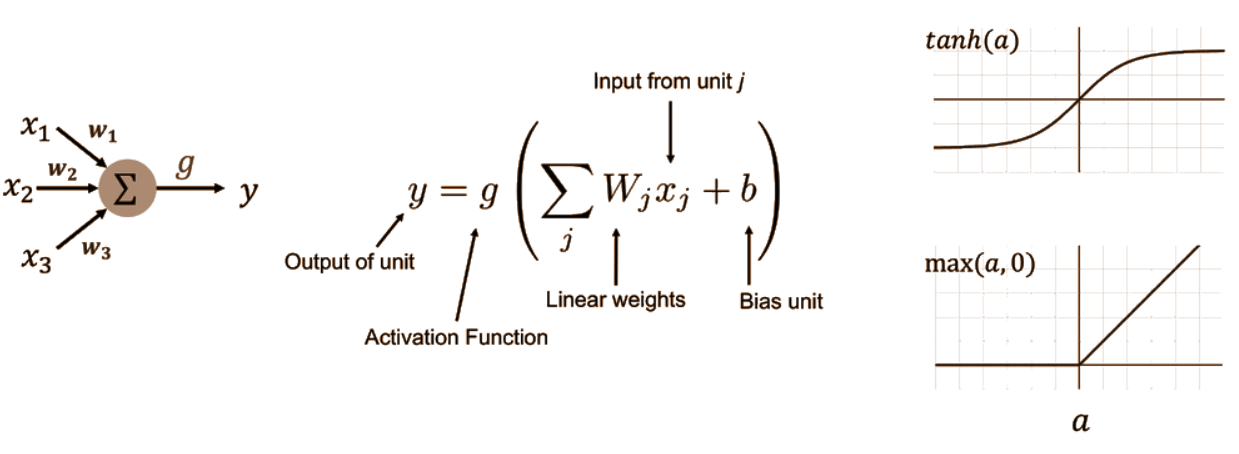
\includegraphics[width=1\linewidth, scale=0.9]{figures/intro/neuron.png}
   \caption[Artificial Neuron]{Artificial Neuron and common activation functions}
    \label{fig:neuron}
\end{figure}


When multiple of neurons are connected in a layer to all the inputs and the output of these neurons are used as input to another set of neurons, then the structure is called as Neural Network. This is shown in the figure ~\ref{fig:ann}. In this network $x_1$ and $x_2$ are the inputs to the network. $f_1(e)$, $f_2(e)$ and $f_3(e)$ are the outputs of three neurons in the first layer. They form as the inputs to the second layer. Simillarly $f_4(e)$ and $f_5(e)$ are the outputs of second layer and $f_6(e)$ is the final output which is used to predict the final value - $y$.


\begin{figure}[H]
	\centering
   \includegraphics[scale=0.66]{figures/intro/neural_network_start.bmp}
   \caption[Artificial Neuron]{Artificial Neuron and common activation functions}
   \label{fig:ann}
\end{figure}

\subsection{Learning \label{lbl:learning}}


Learning of Neural Networks is done in four steps --

\begin{enumerate}
	\item Forward pass

During the forward pass the outputs are computed by multiplying the weights $w$ with the inputs (x). Let $w \times x$ be denoted as $e$ and the activation function be denoted as $f$, then output of a layer $f(e)$ would be $f_1(w_1 \times x_1 + w_2 \times x_2)$. 
If we consider the network shown in figure ~\ref{fig:ann}, then a single forward pass would be as depicted in the figure ~\ref{fig:forward}.

\begin{figure}[H]
	\centering
   \includegraphics[scale=0.66]{figures/intro/forward.bmp}
   \caption[Forward pass]{Computation of a forward pass in a neural network}
   \label{fig:forward}
\end{figure}

	\item Compute error

Error is computed once the model has predicted its output ($y$). Let $z$ be the true output for the given data points. 
Error function or the loss function takes in the predicted value ($y$) and the true value ($z$) and returns some numeric value.
This function is task specific and is different for different tasks. For simplicity let's assume a simple difference, then the error $\delta$ is $z-y$, as shown in the figure ~\ref{fig:error}.

\begin{figure}[H]
	\centering
   \includegraphics[scale=0.66]{figures/intro/error.bmp}
   \caption[Compute error]{Computation of error in a neural network}
   \label{fig:error}
\end{figure}


	\item Backward pass

Backward pass is a phase where error with respect to every neuron is computed. Error at a given layer is the proportion of the error contributed by that layer wrt to the total error. In order to compute error for layer $l$ we need to know error at layer $l+1$. 
Thus, it is computed from layer layer to the first layer and hence called Backward pass. For the networks shown above, error at neuron $2$ is weighted sum of errors at neuron $4$ and $5$. This is shown in the figure ~\ref{fig:error2}.

\begin{figure}[H]
	\centering
   \includegraphics[scale=0.66]{figures/intro/error2.bmp}
   \caption[Backward pass]{Backward pass of the error in a neural network}
   \label{fig:error2}
\end{figure}


	\item Weight update

Final step is to use the error at each neuron to change the weights. Current weight is changed by product of three values - error at the current neuron ($\delta$), gradient of the output wrt to the input at that node ($\frac{df(e)}{de}$)and the output $y$. Generally, this update value is too large and needs to be scaled. This scaling parameter ($\eta$) is called as the \textbf{learning rate} and is generally a hyper-parameter of the network. This step is shown in the figure ~\ref{fig:weight_update}.

\begin{figure}[H]
	\centering
   \includegraphics[scale=0.66]{figures/intro/weight_update.bmp}
   \caption[Weight Update]{Update of weights in a neural network}
   \label{fig:weight_update}
\end{figure}


\end{enumerate}

\section{Introduction to Convolutional Neural Networks}

Convolutional Neural Network (CNN) are like standard neural networks except that not all neurons are connected to every input. 
Only local neighbourhood of inputs are shared for some set of neurons as depicted. Figure ~\ref{fig:cnn} shows the difference between standard Neural Networks (left) and Convolutional Neural Neworks (right).

\begin{figure}[H]
	\centering
   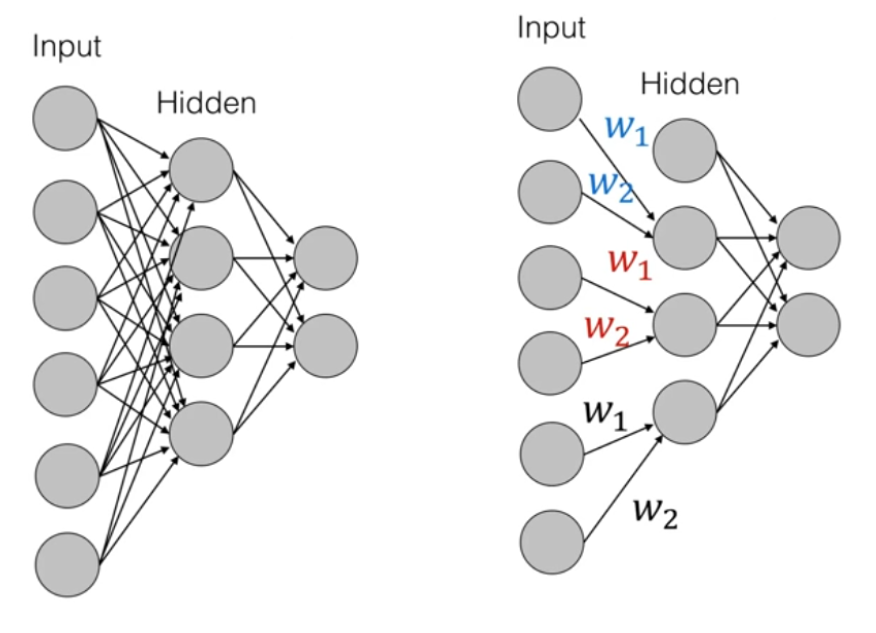
\includegraphics[scale=0.46]{figures/intro/cnn.png}
   \caption[Convolutional Neural Network]{Difference between Standard Neural Network (left) and Convolutional Neural Network (Right)}
   \label{fig:cnn}
\end{figure}

\subsection{Convolution}

While figure ~\ref{fig:cnn} shows CNN in one-dimensional input, it is most widely used with images which are 2-D.
For 2-D data the local inputs shared are a smaller 2-D window in the given image. 
In order to compute the output a smaller 2-D weights (filter) is convolved across the image. 
Generally, this leads to 2-D output but with slighly smaller spatial dimensions due to lack of enough values during convolving at the extreme points. This kind of convolution is called as 'VALID' convolution. In order to achieve the same spatial output the input can be padded wit zeros. This kind of convolution is commonly referred to as 'SAME' convolution. An example of VALID 2-D convolution is shown in the figure ~\ref{fig:cnn2d}. Resulting outputs are called as activation maps. If a layer learns $k$ filters, then there are $k$ activation maps as the output.


\begin{figure}[H]
	\centering
   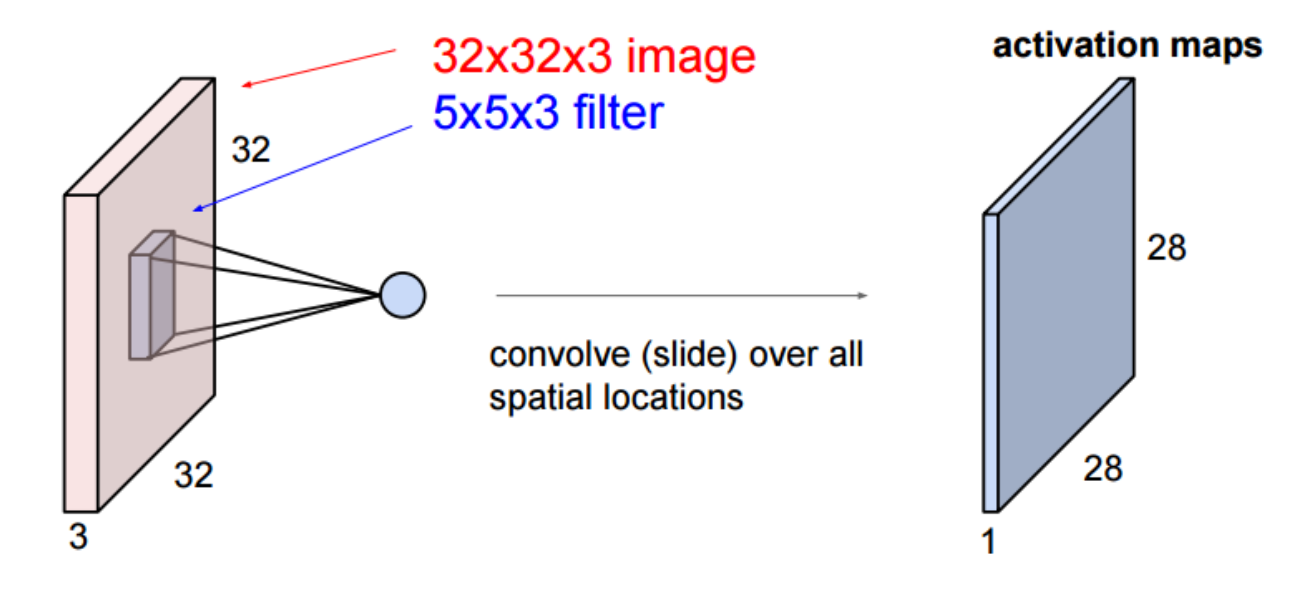
\includegraphics[scale=0.39]{figures/intro/cnn2d.png}
   \caption[2-D Convolution]{VALID 2-D Convolution}
   \label{fig:cnn2d}
\end{figure}

\subsection{Pooling}

Convolutional Neural Networks take in images of some size $H \times W$ and generally, output fixed scalar values in $\mathbb{R}^n$, where $n << H, W$. This often necessitates decreasing the dimensions of the activation maps signficantly (much more than the loss of edges due to VALID convolution). One common technique used to decrease the spatial dimensions is to pool the values within a smaller window. For all values in the window of $h \times w$ is replaced by a single value. Quite often the aggregate function used is the \textbf{max} operation however some models also use averag of the values. Pooling operation is depicted in the figure ~\ref{fig:pool}. In this example pooling window is of the size $2\times2$, which results in the activation halfing in spatial dimensions. 
It is important to note that Pooling does not add any learnable parameters to the network and is often used to reduce the dimensions of the intermediate features.

\begin{figure}[H]
	\centering
   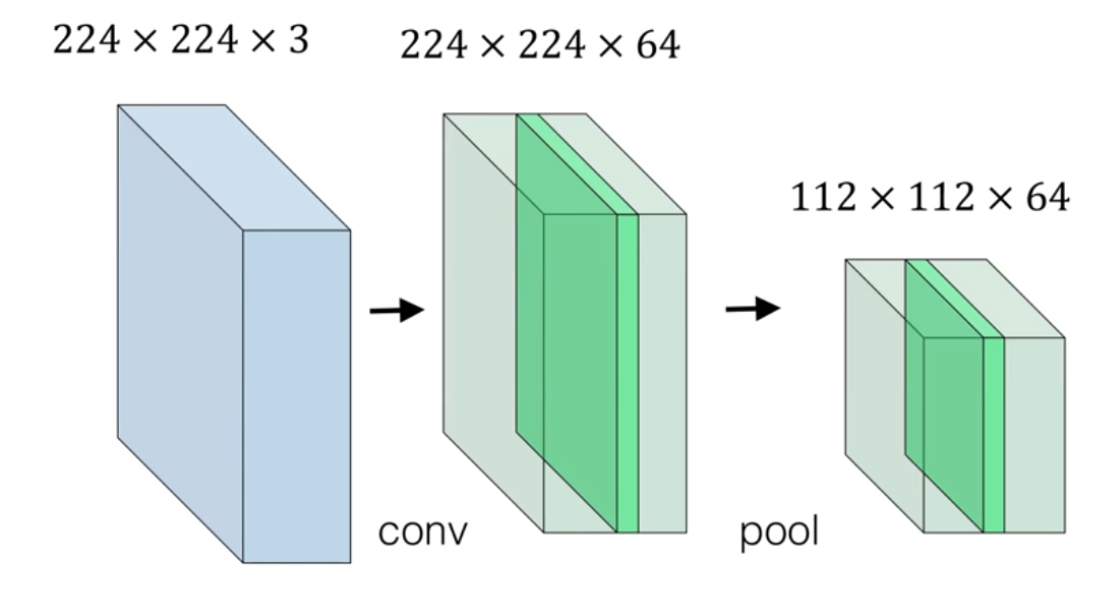
\includegraphics[scale=0.30]{figures/intro/pool.png}
   \caption[Pooling]{Pooling}
   \label{fig:pool}
\end{figure}

\subsection{Normalization}

It is common in Convolutional Neural Networks to include a normalization layer. Normalization layer attempts to rescale the activation values to certain parameters. This is often necessitated due to high variance in the natural images. It has also been shown that normalizing activations leads to faster convergence and sometimes improved performance. In recent times Batch Normmalization has become the preferred choice. If $x$ is the input data and let $\mu$ be the mean of all the activations of the data and $\sigma$ be the standard deviation of the data. Batch normalization first scales the value by subtracting the mean ($\mu$) and dividing by standard deviation $\sigma$. It then adds two learned parameter $\beta$ and $\gamma$, which are used to shift and scale the activations. Thus,

$$
BN(x) = \frac{x-\mu}{\sigma} \gamma + \beta
$$

\subsection{Hierarchical Features}
It has been shown that stacking multiplie layers of convolution operation interspread with pooling leads to learning of hierarchical features. These features become more high-level (semantic) as the layer depth increases. This allows model to learn the semantics in the image and use that to accomplish tasks like classification and detection. Figure ~\ref{fig:features} shows example of filters learned at different depths. One can see that the high-level features are generally observed at filters from higher depth (box on the right) and they look to be formed using the filters from earlier layer (box in the middle), which in turn seems to be compiled from first layer features (left). It has also been shown that first layer filters correspond to edge detectors and gabor filters.

\begin{figure}[H]
	\centering
   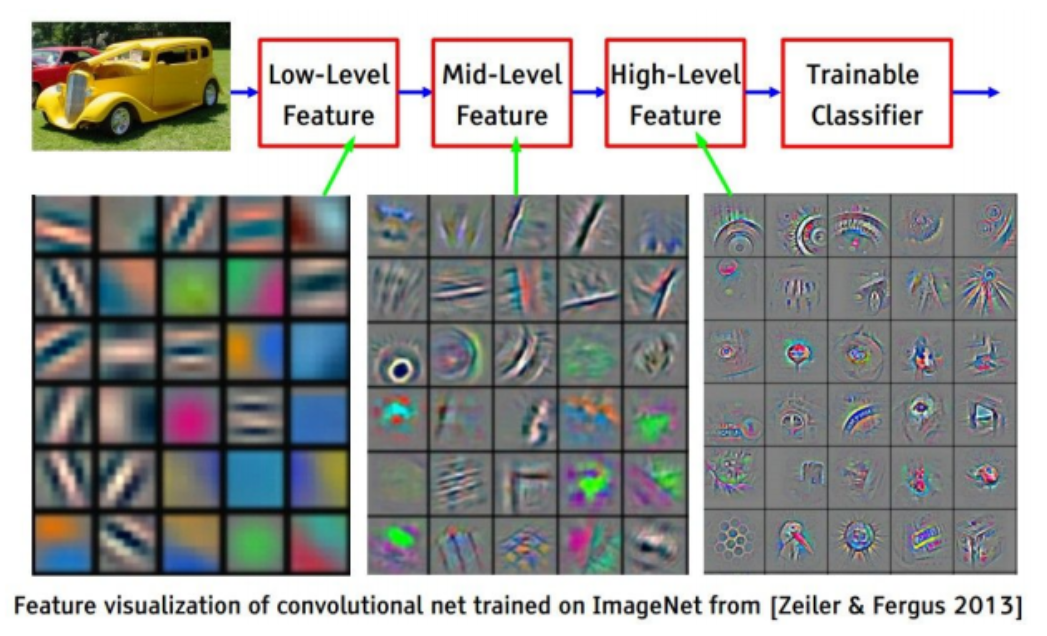
\includegraphics[scale=0.36]{figures/intro/features.png}
   \caption[Hierarchy of features]{Hierarchy of features in CNN}
   \label{fig:features}
\end{figure}

Training of Convolutional Neural Networks is done simillarly to standard Neural Networks as shown in the section ~\ref{lbl:learning}. However, in practice it has been found that training a CNN with many layers is difficult due to vanishing of gradients (backward pass). Several improvements have been suggested to overcome the problem, augment loss term at intermediate depths (Inception Network) ~\cite{Szegedy2016RethinkingTI}, residual skip connections ~\cite{he2016deep}, Highway Networks ~\cite{srivastava2015highway} etc. In depth discussion of these topics are beyond the scope of this manuscript. Reader is advised to refer to the relevant cited works.
